\documentclass[letterpaper, 10pt, conference]{ieeeconf}
\IEEEoverridecommandlockouts
\overrideIEEEmargins

\usepackage[utf8]{inputenc}
\usepackage{amsmath,amssymb}
\usepackage{graphicx}
\usepackage{booktabs}
\usepackage{hyperref}
\usepackage{xcolor}
\usepackage{textcomp}
\usepackage{tikz}
\usepackage{pgfplots}
\usepackage{float}
\usepackage{dblfloatfix}
\pgfplotsset{compat=1.18}
\usetikzlibrary{positioning, arrows.meta, calc, fit, backgrounds}

\title{Bootstrapping Humanoid Foundation Models from Internet-Scale Video}

\author{Anonymous}

\begin{document}

\maketitle

\begin{abstract}
We present a fully open and reproducible pipeline for converting internet-scale human video into training data for humanoid robot control. Our automated pipeline spans person detection, tracking, 2D-to-3D pose lifting, programmatic continuity checks, re-tracking with a vision-language oracle, judgment by a 235B vision-language model, 22-degree-of-freedom joint angle extraction, and instruction caption generation. Starting from $\sim$650K Kinetics-700 videos, the pipeline yields two distributable training sets: \textbf{movement-strict-164} (164,390 clips that pass both programmatic continuity checks and a 235B VLM verdict on skeleton-overlay quality, our highest-quality release) and \textbf{movement-287} (286,890 clips that pass the VLM verdict alone, retaining slower or smaller-bbox activities). Each clip pairs video frames with 3D poses, joint angles, and natural language instructions. The pipeline is validated against motion-capture ground truth and can be applied to any video source.

To demonstrate the datasets' utility, we train MIMIC (Motion Imitation from Massive Internet Clips), a 4.0B-parameter vision-language-action model for full-body humanoid control trained on movement-strict-164. A vision-language backbone conditions a 24-layer diffusion transformer action head that predicts 1.6\,s (16 timesteps) of continuous joint angle trajectories. MIMIC achieves 39.8\textdegree{} RMSE over 22 joints across 1.5\,s of prediction, outperforming both static and linear extrapolation baselines with a 5.3\% advantage on high-motion clips. The model-versus-static gap widens by an order of magnitude compared to a 325K-clip ablation model trained on the unfiltered first-pass output of the same pipeline (1.2\textdegree{} vs 0.1\textdegree{} on average; 3.2\textdegree{} vs 1.7\textdegree{} on high-motion), while training time falls from 14 days to under 6 days on the same hardware. A second model trained on movement-287 matches MIMIC on long-horizon RMSE and produces sharper short-horizon predictions. We observe a consistent pattern across both models: cyclical and repeated activities (pull-ups, squats, jumping rope) predict much more accurately than complex multi-step movements, suggesting that further coverage of long, compositional actions would yield additional gains. Unlike prior humanoid VLAMs that depend on proprietary teleoperation data and large-scale compute infrastructure, our entire system (data pipeline, re-tracking, VLM judging, training, and inference) runs on consumer GPUs. All code, both filtered datasets, and model weights are publicly released.
\end{abstract}

%==============================================================================
\section{Introduction}
%==============================================================================

Vision-language-action models (VLAMs) have emerged as a promising paradigm for robot learning: given a camera image and a natural language instruction (e.g., ``raise both arms overhead''), a VLAM directly outputs the motor commands needed to execute that instruction, unifying perception, language understanding, and motor control in a single model. Recent systems such as RT-2~\cite{rt2}, OpenVLA~\cite{openvla}, $\pi_0$~\cite{pi0}, and GR00T N1~\cite{groot} have demonstrated impressive generalization capabilities, particularly for robotic manipulation tasks.

However, extending VLAMs to \emph{full-body humanoid control} presents unique challenges. Humanoids have significantly more degrees of freedom than typical manipulators (17+ joints vs.\ 6--7), require whole-body coordination, and must handle dynamic balance, making the action space both higher-dimensional and more tightly constrained. Prior work on full-body control from language, such as MotionGPT~\cite{motiongpt} and UH-1~\cite{uh1}, operates in \emph{open-loop}: given a text instruction, these models produce motion sequences without visual feedback, and cannot react to environmental changes or correct for drift.

The recent Helix~\cite{helix} and GR00T N1--N1.6~\cite{groot,groot_n15,groot_n16} systems demonstrate closed-loop humanoid VLAMs, but all rely on proprietary robotic teleoperation data and, in Helix's case, closed-source models. This creates a barrier for research: without access to humanoid robots and teleoperation infrastructure, researchers cannot reproduce or build upon these systems.

\textbf{Our approach.} We address this by training a closed-loop humanoid VLAM entirely from \emph{human video data}. Internet-scale human video contains rich demonstrations of full-body motion that, when properly processed, can serve as training data for humanoid imitation learning. Our contributions are:

\begin{enumerate}
    \item \textbf{Open Pipeline:} An end-to-end pose extraction and curation pipeline (detection, tracking, 2D$\to$3D lifting, programmatic continuity filters, re-tracking with a vision-language oracle, judgment by a 235B vision-language model, VLM captioning) that converts raw internet video into training-ready data, applicable to any video source.
    \item \textbf{Open Datasets:} Two distributable training sets, movement-strict-164 (164K clips, prog $\land$ VLM) and movement-287 (287K clips, VLM only), each with extracted 3D poses, joint angles, and instruction-style captions from Kinetics-700.
    \item \textbf{Open Model:} MIMIC, a VLAM with trained weights that takes visual observations and language instructions as input and outputs continuous 22-DoF joint angle trajectories.
    \item \textbf{Open Infrastructure:} Complete training, re-tracking, and VLM-judging code that runs on consumer GPUs.
\end{enumerate}

\begin{table*}[t]
\centering
\caption{Comparison of vision-language-action models. MIMIC is the only humanoid VLAM that is fully open-source, trains from freely available internet video, and runs on consumer hardware.}
\label{tab:vlam_compare}
\resizebox{\textwidth}{!}{%
\begin{tabular}{lccccccc}
\toprule
\textbf{Model} & \textbf{Params} & \textbf{Embodiment} & \textbf{DoF} & \textbf{Closed-Loop} & \textbf{Open Source} & \textbf{Data Source} & \textbf{Training Compute} \\
\midrule
RT-2~\cite{rt2} & 55B & Arm & 7 & \checkmark & \texttimes & Robot teleop & Datacenter \\
Octo~\cite{octo} & 93M & Arm & 7 & \checkmark & Weights+Code & Robot teleop & 8$\times$A100 \\
OpenVLA~\cite{openvla} & 7B & Arm & 7 & \checkmark & Weights+Code & Robot teleop & 16$\times$A100 \\
$\pi_0$~\cite{pi0} & 3B & Arm & 7+ & \checkmark & \texttimes & Robot teleop & Datacenter \\
UH-1~\cite{uh1} & N/R & Humanoid & 52 & \texttimes & Scripts only & Human video & N/R \\
GR00T N1~\cite{groot} & 2.2B & Humanoid & 52 & \checkmark & Weights only & Teleop + MoCap & $\sim$50K H100-hrs \\
GR00T N1.5~\cite{groot_n15} & 3.0B & Humanoid & 52 & \checkmark & Weights only & Teleop + human video & 1K H100s \\
Helix~\cite{helix} & $\sim$7B & Humanoid & 35 & \checkmark & \texttimes & 500h teleop & Datacenter \\
\midrule
\textbf{MIMIC (Ours)} & 4.0B & Humanoid & 22 & \checkmark & All (W+C+D) & Internet video & 4$\times$RTX ($\sim$576 hrs) \\
\bottomrule
\end{tabular}%
}
\end{table*}

%==============================================================================
\section{Related Work}
%==============================================================================

\subsection{Vision-Language-Action Models}

VLAMs extend vision-language models (VLMs) to output robot actions conditioned on visual observations and language instructions. RT-2~\cite{rt2} first demonstrated this paradigm by fine-tuning a VLM to output discretized actions. Subsequent work has explored various architectural choices: OpenVLA~\cite{openvla} provides an open-source 7B-parameter alternative; $\pi_0$~\cite{pi0} introduces flow matching for continuous action generation; and Octo~\cite{octo} and TinyVLA~\cite{tinyvla} explore efficient architectures for resource-constrained deployment.

\textbf{Recent developments:} The field has advanced rapidly. Physical Intelligence released $\pi_{0.5}$~\cite{pi05} with co-training on heterogeneous tasks and $\pi_0$-FAST~\cite{pi0fast} with frequency-space action tokenization. Google DeepMind introduced Gemini Robotics 1.5~\cite{gemini15} with a Motion Transfer mechanism for multi-embodiment learning. SmolVLA~\cite{smolvla} provides a compact 450M-parameter open-source alternative using flow matching. OpenVLA-OFT~\cite{openvla_oft} integrates action chunking, boosting success from 76.5\% to 97.1\% on LIBERO. A2A~\cite{a2a} achieves single-step inference (0.56ms) by initializing from prior actions.

\subsection{Full-Body Motion from Language}

A parallel line of work generates full-body human motion from text descriptions. MotionDiffuse~\cite{motiondiffuse} and MotionGPT~\cite{motiongpt} use diffusion and GPT-style architectures, respectively, to generate motion sequences. However, these approaches are \emph{open-loop}: they do not condition on visual observations and cannot adapt to environmental feedback.

UH-1~\cite{uh1} is most similar to our approach: it processes Kinetics videos to create the Humanoid-X dataset of 20M poses with text descriptions. However, UH-1 only provides scripts to \emph{recreate} the dataset (not the dataset itself), uses simpler pixel-wise motion detection (vs.\ our pose-based filtering), operates in open-loop, and does not release model weights.

\subsection{Learning from Human Video}

Several works explore learning robot control from human demonstrations. R3M~\cite{r3m} learns visual representations from human video. EgoVLA~\cite{egovla} pretrains on egocentric human manipulation data and uses inverse kinematics to retarget to robots. mimic-video~\cite{mimicvideo} pairs internet-scale video models with flow matching action decoders, achieving 10$\times$ better sample efficiency than standard VLAs. WholeBodyVLA~\cite{wholebodyvla} learns latent actions from action-free egocentric videos through a Latent Action Model. SONIC~\cite{sonic} scales motion tracking to 42M parameters on 700 hours of data to produce natural humanoid control. Our work differs by directly extracting 3D pose from third-person video, requiring no egocentric data, paired demonstrations, or simulation.

\subsection{Humanoid VLAMs}

GR00T N1~\cite{groot} pairs an Eagle-2 VLM with a 16-layer DiT flow matching head (2.2B parameters total), trained on teleoperation, motion capture, and synthetic data ($\sim$50K H100-hours). NVIDIA released open weights and fine-tuning code under a non-commercial license, though pretraining data remains proprietary. GR00T N1.5~\cite{groot_n15} (3.0B) replaces Eagle-2 with an improved VLM and introduces a FLARE loss that aligns future latent representations, enabling learning from human video alongside teleoperation data. GR00T N1.6~\cite{groot_n16} (3.3B) doubles DiT capacity to 32 layers and switches to state-relative action prediction for smoother trajectories. Our architecture follows N1's dual-system design but trains entirely from internet video and requires $\sim$87$\times$ less compute.

Helix~\cite{helix} uses a 7B VLM at $\sim$8Hz conditioning an 80M visuomotor policy at 200Hz, trained on $\sim$500 hours of teleoperation. Neither release includes weights, code, or data. All of these systems rely on proprietary teleoperation data, simulation, or motion capture; our work trains from freely available internet video alone.

%==============================================================================
\section{Dataset Construction}
%==============================================================================

Our dataset pipeline processes raw Kinetics-700 videos through two stages. The first stage (Sections~\ref{sec:filtering} and earlier) handles ingestion, person detection and tracking, 2D pose estimation, 3D pose lifting, and programmatic quality filtering, producing an intermediate corpus of 325,036 tracked clips. The second stage (Section~\ref{sec:retracking}) re-tracks each clip using a vision-language oracle to pick the correct subject and a stricter IoU tracker to maintain identity, then judges every clip with a 235B vision-language model on rendered skeleton overlays. We release the resulting two filtered datasets, movement-strict-164 and movement-287, and use them for all model training in this paper. Instruction captions (Section~\ref{sec:captioning}) are generated once and reused across both subsets.

\subsection{Data Source Selection}

We selected Kinetics-700 as our primary data source for several reasons: (1) large scale (650K+ videos across 700 action classes); (2) diversity of human activities; (3) ``in-the-wild'' recording conditions that improve model robustness; and (4) it provides prefiltering to save compute time by limiting to videos of human action compared to general internet video.

\textbf{NTU RGB+D 120 for Validation.} While Kinetics provides scale and diversity, it lacks ground-truth 3D pose annotations. We use NTU RGB+D 120~\cite{ntu120} to validate our pose extraction pipeline. NTU RGB+D 120 contains 114K video clips with synchronized RGB, depth, and skeleton annotations captured via Kinect sensors across 120 action classes. However, NTU's controlled lab environment (uniform backgrounds, fixed camera positions) makes it poorly suited as training data. We therefore use NTU exclusively for \emph{validating} our pose extraction pipeline's accuracy before applying it to Kinetics.

\subsection{Person Detection and Tracking}

Videos often contain multiple people, camera cuts, and scene transitions. We must reliably track a single target person throughout each clip. Getting this right required iteration. Early approaches frequently swapped identities during posture changes and occlusions, producing corrupted pose sequences.

\textbf{Detection.} We use YOLOv8x for person detection, running on frames downsampled to 480p at $\sim$10fps (matching our target pose frequency), with batch detection of 32 frames on GPU.

\textbf{Tracking.} We employ ByteTrack~\cite{bytetrack} with Kalman filter motion prediction. The key insight was tuning the IoU matching threshold: the default ($0.8$) is too strict for activities with large frame-to-frame posture changes (e.g., gymnastics, dancing), causing frequent track fragmentation. Lowering \texttt{match\_thresh} to $0.3$ allows the tracker to maintain identity through rapid pose changes while the Kalman filter bridges brief occlusions. We retain lost tracks for 30 frames and use two-stage association following the original ByteTrack design.

\textbf{Target Selection.} When multiple people are detected, we select the primary target based on: (1) largest average bounding box area; (2) longest continuous track duration; (3) consistency of motion. We reject clips where tracking switches between people or where the primary target disappears for extended periods.

\textbf{Hard Cut Detection.} Scene transitions invalidate temporal continuity assumptions. We detect hard cuts by computing histogram correlation between consecutive frames; correlation below 0.4 indicates a likely scene change. Clips containing hard cuts are split at cut boundaries or rejected.

\begin{figure*}[t]
\centering
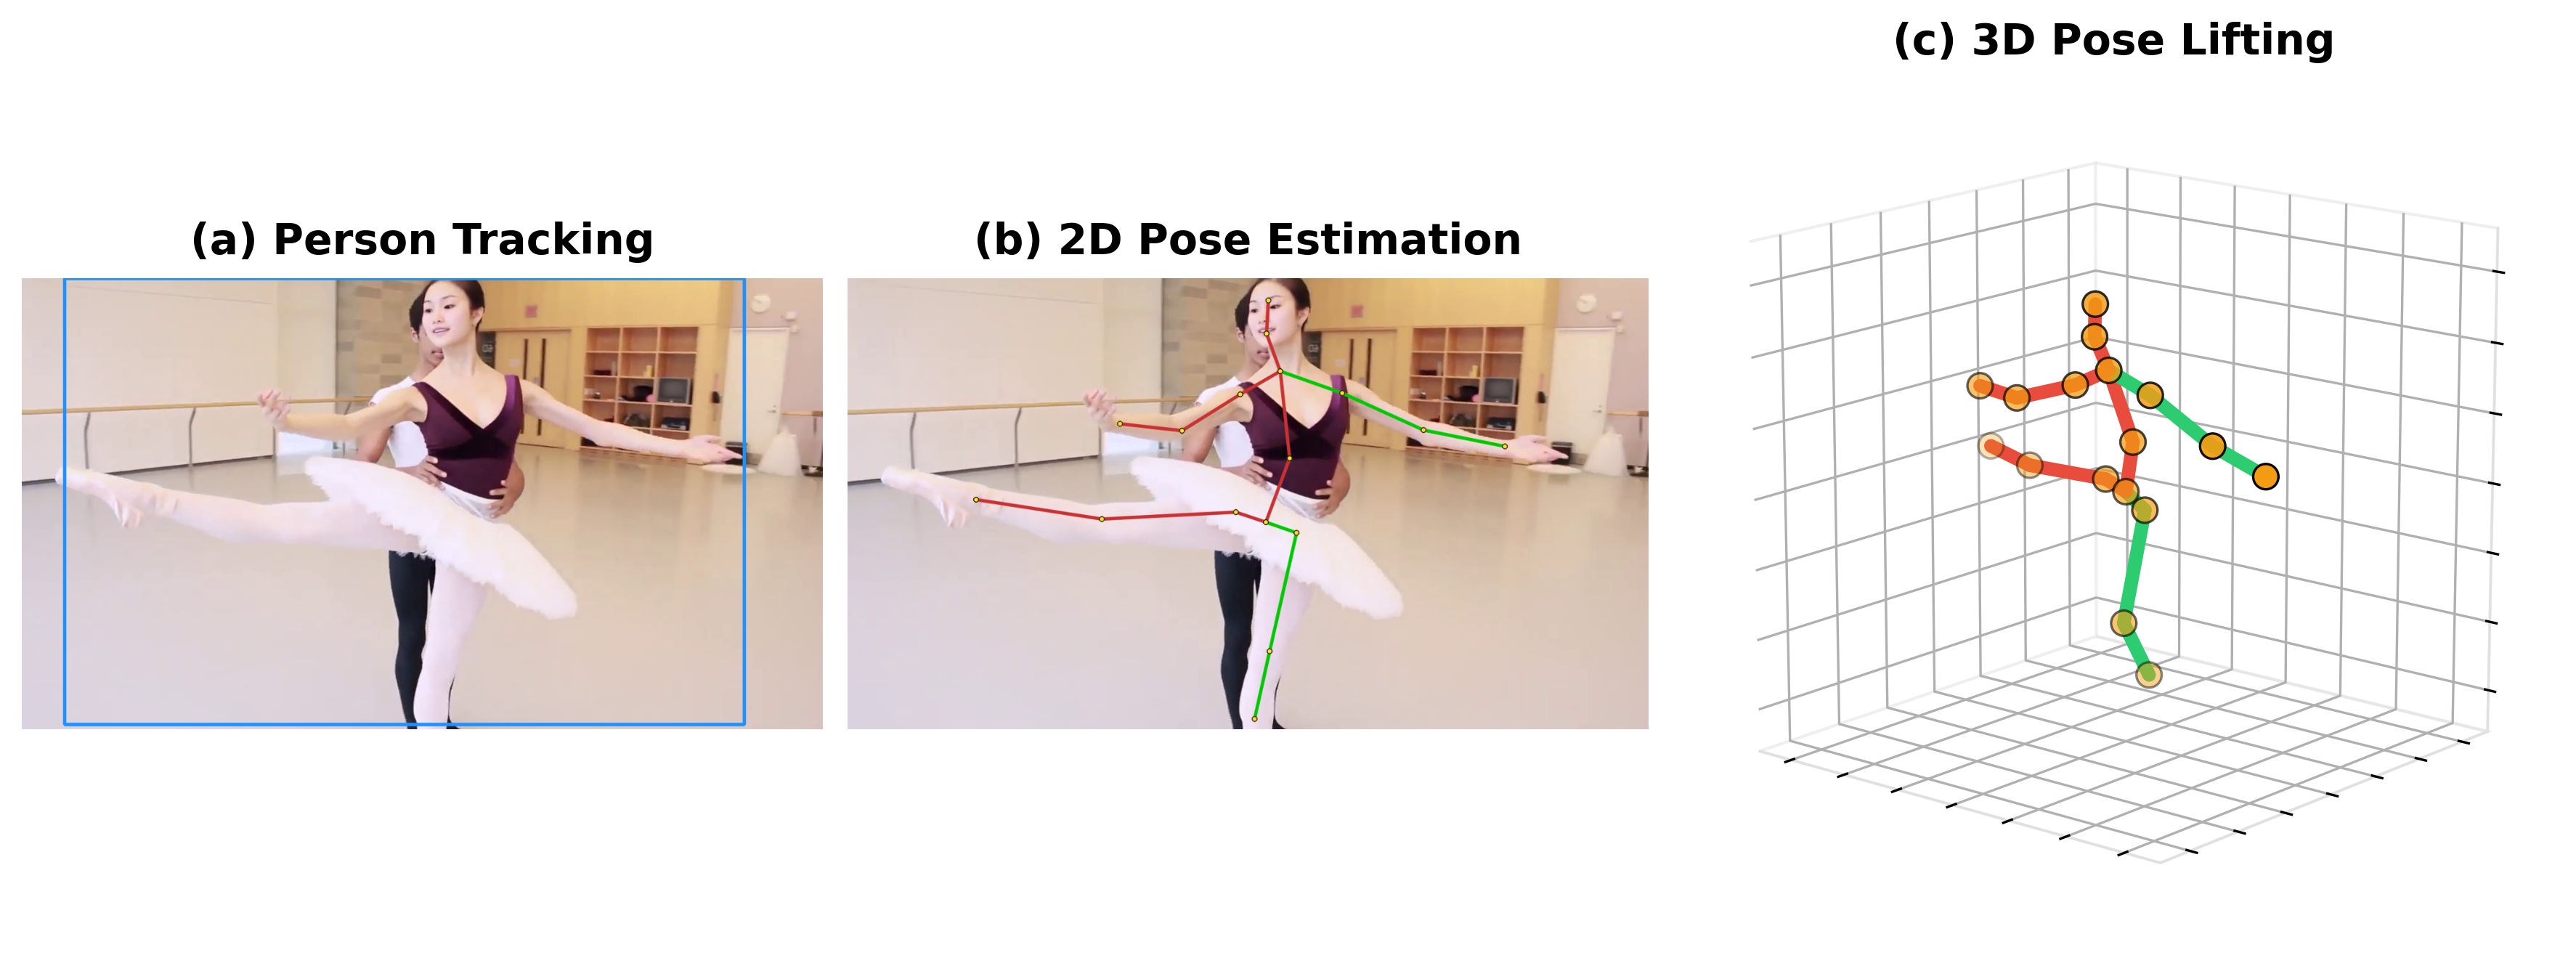
\includegraphics[width=\textwidth]{figures/pipeline_figure.png}
\caption{Overview of the pose extraction pipeline applied to a Kinetics-700 video clip. (a) Person tracking localizes the subject via bounding box detection. (b) 2D pose estimation extracts 17 H36M keypoints using ViTPose. (c) 3D pose lifting via MotionAGFormer produces temporally consistent 3D joint positions, from which 22-DoF joint angles are computed via inverse kinematics.}
\label{fig:pipeline}
\end{figure*}

\subsection{Pose Estimation}

\textbf{2D Pose.} We use ViTPose-Large~\cite{vitpose}, a vision transformer-based pose estimator pretrained on COCO and fine-tuned on multiple pose datasets. ViTPose produces 17 COCO-format keypoints per frame with confidence scores. We crop frames to tracked bounding boxes (with 10\% padding) before pose estimation for improved accuracy.

\textbf{3D Lifting.} Monocular 3D pose estimation remains challenging due to depth ambiguity. We employ MotionAGFormer~\cite{motionagformer}, a graph-attention transformer trained on Human3.6M that lifts 2D pose sequences to 3D, processing 243-frame clips for temporal smoothing and physical plausibility constraints.

To validate our pipeline, we evaluate on 200 randomly sampled NTU RGB+D 120 clips, comparing our monocular predictions against Kinect ground truth. Converting both to our 22-DoF joint angle representation, the pipeline achieves a joint angle RMSE of 74.6\textdegree{} (median 74.6\textdegree{}, std 7.3\textdegree{}) with zero pipeline failures. This gap reflects compounding factors: NTU's 25 Kinect joints map only approximately to H3.6M's 17-joint skeleton, Kinect depth sensors have 20--50mm noise, and MoCap marker data captures fundamentally different body geometry than Kinect's depth-fitted skeleton.

\textbf{Coordinate Normalization.} Raw 3D poses are in arbitrary camera-relative coordinates. We normalize to a canonical representation: root (pelvis) at origin, facing direction aligned to Z-axis, height-normalized to unit scale.

\textbf{Joint Angle Conversion.} For training, we convert 3D joint positions to 22 joint angles (Section~\ref{sec:action_rep}). This representation is more suitable for humanoid control, as robots are actuated in joint space rather than Cartesian space.

\subsection{Quality Filtering}
\label{sec:filtering}

Raw pose extractions contain substantial noise from detection failures, tracking errors, and pose estimation artifacts. We apply multi-stage filtering:

\textbf{Body Coverage.} We require at least 3 of 5 ``core'' joints (nose, shoulders, hips) to be detected with confidence $>0.3$ in at least 40\% of frames. Clips failing this criterion typically contain severe occlusions or non-frontal views.

\textbf{Motion Significance.} We reject clips with insufficient motion, as they provide little training signal. Unlike UH-1's pixel-wise grayscale differencing, we compute motion in \emph{pose space}: average frame-to-frame joint displacement, normalized by approximate body scale. Additionally, we check for \emph{pose variation}: static poses held across frames (e.g., standing still) are valid if joint configurations differ. This allows activities like yoga poses while rejecting genuinely static clips.

\textbf{Tracking Consistency.} We measure tracking quality via: (1) IoU between consecutive bounding boxes (low IoU indicates jumps); (2) bounding box size ratio changes (sudden size changes indicate scale inconsistency or track switches). Clips exceeding 10\% of frames with IoU $<0.1$ and size ratio $>2\times$ are rejected.

Of the original $\sim$650K Kinetics-700 videos, $\sim$325K clips ($\sim$51\%) survive stage-1 filtering and form the intermediate corpus that stage 2 re-tracks and judges. Primary stage-1 attrition causes are: multi-person scenes without a clear dominant subject ($\sim$20\%), detection failures in challenging viewpoints ($\sim$15\%), and videos no longer available for download ($\sim$14\%). Among surviving clips, $\sim$46K (13.9\%) contain detected hard cuts and are split at cut boundaries. Pose sequences average 242 frames (median 283, range 20--301), corresponding to $\sim$24s of motion data at 10Hz after temporal subsampling.

\subsection{Re-tracking and VLM-Judged Filtering}
\label{sec:retracking}

The programmatic filters above remove most catastrophic failures but cannot detect a class of semantic errors that resemble valid tracking: subject swaps onto similarly-sized co-actors, tracking that visually drifts to a different person mid-clip, or clips where the labeled action is actually performed by someone other than the tracked subject. We address these in a second pass that combines a stricter re-tracker with a VLM judge.

\textbf{Re-tracking pipeline.} For each clip in the stage-1 corpus, we re-detect candidates with YOLOv8x across five evenly sampled frames, then pool detections into a candidate set rendered with numbered boxes onto the busiest anchor frame. A Qwen3-VL oracle selects the subject performing the labeled action. From that anchor, a sticky IoU tracker (threshold 0.5, size-ratio guard 2.5$\times$, three-miss tolerance) propagates forward and backward, breaking on persistent loss rather than drifting. The clip is trimmed to the longest valid run containing the anchor, with hard cuts re-detected on the trimmed frame range, and residual interior bounding-box gaps interpolated. ViTPose and MotionAGFormer then re-run from the corrected crops. The pipeline aborts on clips where no run of at least 20 frames contains the anchor, isolating clips that are inherently unfixable.

\textbf{VLM-judged verdict.} Each clip (original or re-tracked) is rendered with the chosen skeleton overlay at six sampled frames and submitted to Qwen3-VL-235B-A22B-Thinking, served locally via vLLM across 4 GPUs. The judge returns two booleans: \emph{tracking\_consistent} (the same clearly-visible person is cleanly tracked throughout, with no scene cuts or skeleton drift onto other people) and \emph{motion\_matches} (the tracked person is performing the labeled action class). We refer to these jointly as the VLM-good verdict. We tuned the prompt and selected the 235B Thinking model after sweeping smaller variants on a 40-clip manually-labeled set; the 235B judge achieves 92.5\% agreement with human labels.

\textbf{Composite verdict and release.} For each of the 325,036 clips in the stage-1 corpus, we record both the programmatic verdict from stage 1 and the VLM-good verdict from stage 2, replacing the tracking data with the re-tracked NPZ when the re-tracker succeeded (193,277 clips) and falling back to the original stage-1 tracking otherwise (131,759 clips). This yields two distributable filtered subsets summarized in Table~\ref{tab:filtered}.

\begin{table}[h]
\centering
\caption{Filtered training sets produced by stage 2. Strict requires both programmatic and VLM verdicts; vlm-good requires only the VLM judge. The intermediate 325K corpus is reported for reference and is not used for training in this paper.}
\label{tab:filtered}
\begin{tabular}{lrr}
\toprule
\textbf{Subset} & \textbf{Clips} & \textbf{\% of intermediate} \\
\midrule
Intermediate stage-1 corpus & 325{,}036 & 100.0\% \\
\textbf{movement-287} (vlm-good) & 286{,}890 & 88.3\% \\
\textbf{movement-strict-164} (vlm-good $\land$ prog) & 164{,}390 & 50.6\% \\
\bottomrule
\end{tabular}
\end{table}

\textbf{Scale-out cost.} Judging all 325,036 clips with the 235B Thinking model took 4.9 days at 33 clips per minute on 4 GPUs with batched concurrent requests. Re-tracking the 217,122 clips on which either signal disagreed took 3.4 days at 44 clips per minute split across the 4 GPUs (one tracker per GPU, local Qwen oracle). Re-judging the retracked subset took an additional 2.9 days. Total wall-clock for the data refinement pass: roughly 11 days for all 325K clips, end to end. Zero VLM errors over the entire 519,148 judgment calls.

\subsection{Instruction Caption Generation}
\label{sec:captioning}

At inference time, a VLAM receives a natural language instruction describing the desired motion and must translate it into joint-angle commands. Our training captions must therefore resemble the instructions a robot operator would issue at deployment. We generate these using Qwen3-VL-32B~\cite{qwen3vl}, with prompt engineering that ensures captions describe \emph{physical motions as imperative commands}:

\begin{quote}
\small
``Rewrite only the physical motion as a sequence of imperative commands. Do not mention a person, actor, bounding box, body type, clothing, scene, environment, animals, spectators, or camera. Mention only objects that the action physically interacts with. Do not narrate, summarize, or describe anything. Use only imperative verbs. Start immediately with a command. Format: 1--3 short sentences in pure imperative form.''
\end{quote}

Example output (bowling): ``Bend the knees and hinge at the hips to lower the torso, extend the right arm forward and swing the bowling ball in a smooth arc, then release the ball by rotating the wrist and pushing it down the lane.''

We evaluated several VLMs for caption generation, including Qwen3-VL-8B, Qwen3-VL-32B, and Video-LLaVA, and selected Qwen3-VL-32B-Instruct for its consistent adherence to the imperative-form prompt with fewer hallucinated scene details. Caption coverage is near-complete: 99.998\% of stage-1 clips received valid captions, which are inherited by both filtered subsets.

\subsection{Dataset Statistics}

\begin{table}[h]
\centering
\caption{Dataset statistics for the two released training sets. Strict-164 is the highest-quality subset and is used for our primary released model.}
\label{tab:dataset}
\begin{tabular}{lrr}
\toprule
\textbf{Metric} & \textbf{movement-287} & \textbf{strict-164} \\
\midrule
Total clips & 286{,}890 & 164{,}390 \\
Action classes & 700 & 700 \\
Training samples & 3.34M & 1.86M \\
Validation samples & 174{,}197 & 59{,}677 \\
Joint angle dimensions & 22 & 22 \\
Action horizon & \multicolumn{2}{c}{16 frames (1.6s)} \\
Frame rate & \multicolumn{2}{c}{10 Hz} \\
\bottomrule
\end{tabular}
\end{table}

Each clip yields multiple non-overlapping action windows of 16 frames. Both training sets use a 95\%/5\% train/val split stratified by clip-id hash, preventing leakage at the clip level. We use 5\% rather than 2\% because the clip-id hash distribution skews high enough that a 2\% threshold produces zero validation clips on the filtered subsets.

%==============================================================================
\section{Model Architecture}
%==============================================================================

MIMIC's architecture follows the dual-system design introduced by Helix~\cite{helix} and adopted by GR00T N1~\cite{groot}, scaled to run on consumer hardware.

\subsection{Overview}

The model comprises two components:

\textbf{System 2 (Vision-Language Encoder):} A pretrained VLM (Qwen3-VL-4B) processes visual observations and language instructions, producing latent representations that capture scene understanding and task semantics.

\textbf{System 1 (Action Decoder):} A diffusion transformer converts S2 latents into continuous joint-angle trajectories at 10Hz.

\begin{figure*}[t]
\centering
\includegraphics[width=\textwidth, height=0.4\textheight, keepaspectratio]{figures/oh-vlam-architecture.pdf}
\caption{Model architecture. A pretrained VLM (Qwen3-VL-4B) encodes visual observations and language instructions into latent representations (System 2). These condition a diffusion transformer that generates continuous 22-DoF joint-angle trajectories at 10Hz (System 1). We extract intermediate hidden states from layer 18 of 36 and apply LoRA adapters, keeping base weights and the vision encoder frozen.}
\label{fig:architecture}
\end{figure*}

\subsection{Vision-Language Encoder}

We use Qwen3-VL-4B as the vision-language backbone, selected for its strong performance on visual understanding benchmarks and manageable parameter count. The encoder processes:

\begin{itemize}
    \item \textbf{Visual input:} 4 frames sampled from immediately before the action window, providing temporal context without leaking future poses.
    \item \textbf{Language input:} Instruction caption describing the target motion.
    \item \textbf{Bounding box overlay:} A green rectangle indicating the target person, rendered directly on input frames.
\end{itemize}

Following GR00T N1, we extract hidden states from an intermediate layer (layer 18 of 36) rather than the final layer. For inference, we truncate the Qwen model after layer 18, skipping layers 19--36 entirely, providing $\sim$2$\times$ speedup with minimal quality degradation.

\textbf{Parameter Efficiency.} We apply LoRA (rank 128, $\alpha$=128, dropout 0.05) to all attention and MLP layers (\texttt{q/k/v/o\_proj}, \texttt{gate/up/down\_proj}), keeping base weights frozen. The vision encoder remains fully frozen throughout training.

\subsection{Action Representation}
\label{sec:action_rep}

We represent actions as 22-dimensional joint angle vectors, computed via inverse kinematics from H3.6M 3D joint positions:

\begin{itemize}
    \item Spine: 3 DoF (pitch, roll, yaw)
    \item Each hip: 3 DoF + 1 DoF knee (4 DoF $\times$ 2 = 8 DoF)
    \item Each shoulder: 3 DoF + 1 DoF elbow (4 DoF $\times$ 2 = 8 DoF)
    \item Neck: 3 DoF
\end{itemize}

This joint-angle representation directly maps to robot actuation, implicitly encodes kinematic constraints, and is more compact than 17$\times$3 = 51 position dimensions. The model predicts 16 future timesteps at 10Hz (1.6 seconds).

\subsection{Diffusion Action Head}

The action decoder uses flow matching~\cite{flowmatching}, a diffusion variant with simpler training objectives and deterministic inference. Architecture follows DiT (Diffusion Transformer) design:

\textbf{Input sequence:} [state token, 4 future tokens, 16 action tokens] = 21 tokens. The state token encodes current proprioception (22D joint angles); future tokens are learnable embeddings providing planning context (following GR00T); action tokens encode the noisy action trajectory with positional embeddings.

\textbf{Conditioning:} Timestep conditioning via AdaLN (Adaptive Layer Normalization). Cross-attention in each DiT block attends to Qwen hidden states.

\textbf{Architecture details:} Hidden dimension 1536, 24 DiT blocks, 24 attention heads. Two-stage projection from Qwen (2560D $\to$ 1024D $\to$ 1536D) with LayerNorm and SiLU. DeepStack features concatenate early-layer (layer 9) and target-layer (layer 18) Qwen features for multi-scale representations. Training timesteps sampled from Beta(1.5, 1.0), biasing toward lower noise levels.

\textbf{Absolute angle prediction.} The model directly predicts absolute joint angles for each timestep rather than residuals from the current pose (see ablation in Section~\ref{sec:ablations}).

\subsection{Training}

\textbf{Loss:} Flow matching velocity prediction: $\mathcal{L} = \|v_\theta(x_t, t) - (a - \epsilon)\|^2$ where $x_t = t \cdot a + (1-t) \cdot \epsilon$ is the noisy interpolation, $a$ the target actions, $\epsilon \sim \mathcal{N}(0, I)$ noise, and $t \sim \text{Beta}(1.5, 1)$.

\textbf{Training schedule:} We train for 2 epochs. The vision encoder is frozen throughout; the LLM backbone uses LoRA. The DiT action head trains from scratch. Data is augmented with horizontal flips (swapping left/right joints and mirroring instruction text), effectively doubling the dataset. Non-overlapping action windows (stride = action horizon = 16 frames) prevent data leakage between training samples.

\textbf{Hyperparameters:} AdamW optimizer with weight decay 0.01; action head LR $1\times10^{-5}$, LoRA LR $1\times10^{-6}$; batch size 8 per GPU with 16-step gradient accumulation across 4 GPUs (effective batch 512); cosine annealing with warm restarts; gradient clipping at 1.0; mixed-precision bf16.

\textbf{Compute.} Training uses 4$\times$98GB RTX Pro Blackwell GPUs. The strict-164 model trains in 5.9 days ($\sim$566 GPU-hours). The movement-287 sibling model takes 8.8 days. The data preparation pipeline (stage 1 plus stage 2 re-tracking and judging) totals roughly 11 wall-clock days the first time it is run, and is fully reusable across subsequent training runs. End to end on a single workstation, going from raw Kinetics-700 to the strict-164 model takes under 17 days. For comparison, GR00T N1 reports $\sim$50K H100-hours ($\sim$\$100K at cloud rates) for training alone. Peak memory is $\sim$49GB per GPU.

%==============================================================================
\section{Inference and Visualization}
%==============================================================================

\subsection{Inference Pipeline}

Closed-loop inference proceeds as follows:

\begin{enumerate}
    \item Sample 4 frames from current observation window
    \item Encode frames + instruction via Qwen3-VL (early exit at layer 18)
    \item Initialize action trajectory as Gaussian noise
    \item Run single-step Euler ODE integration through the learned velocity field
    \item Extract predicted absolute joint angle trajectory
    \item Execute first action from predicted 16-step trajectory; repeat
\end{enumerate}

\textbf{Latency:} Single-step inference requires only 1 forward pass through the DiT, with the Qwen encoder forward pass dominating latency. End-to-end inference completes well within the 100ms budget for 10Hz control.

\subsection{Evaluation Protocol}
\label{sec:viz}

A challenge for humanoid VLAM research is the lack of accessible simulation environments. Unlike manipulation (which benefits from MuJoCo/Isaac Gym with realistic physics), humanoid simulation at the fidelity required for VLAM evaluation remains an open problem.

We therefore evaluate via \emph{prerecorded video playback}: given a held-out video clip, we feed frames to the model as if they were live observations and compare predicted pose trajectories against ground-truth extracted poses. To qualitatively assess predictions, we project predicted 3D joint positions to 2D via Procrustes alignment against ground-truth keypoints, then overlay predicted skeletons on video frames with temporal opacity gradients.

\textbf{Limitations.} This evaluation has inherent limitations: (1) the model cannot affect the ``environment'' (video playback is fixed); (2) we cannot evaluate recovery from errors; (3) we cannot assess balance or contact dynamics. These limitations motivate future work on humanoid simulation environments (Section~\ref{sec:limitations}).

\subsection{Metrics}

We report:
\begin{itemize}
    \item \textbf{Joint Angle RMSE:} Root mean squared error in radians between predicted and ground-truth joint angles
    \item \textbf{Position MPJPE:} Mean per-joint position error after converting angles to 3D positions (mm)
    \item \textbf{Pipeline Angle RMSE:} Joint angle RMSE between pipeline-extracted and motion-capture ground truth (74.6\textdegree{} on NTU RGB+D 120), representing the training data noise floor
\end{itemize}

%==============================================================================
\section{Experiments}
%==============================================================================

\subsection{DiT Scaling}
\label{sec:scaling}

We train four model variants with increasing diffusion transformer capacity, keeping the Qwen3-VL-4B backbone and LoRA configuration fixed. Table~\ref{tab:scaling} shows consistent improvement with DiT scale up to 24 layers, with no meaningful gain beyond that.

\begin{table}[h]
\centering
\caption{DiT scaling results. All models use Qwen3-VL-4B with LoRA (rank 128). Val loss is flow matching MSE on held-out clips.}
\label{tab:scaling}
\begin{tabular}{lcc}
\toprule
\textbf{Config} & \textbf{Params} & \textbf{Val Loss} \\
\midrule
S: 8L / 512D & 54M & 0.318 \\
M: 12L / 768D & 168M & 0.298 \\
L: 24L / 1536D (final) & 1.28B & \textbf{0.265} \\
XL: 48L / 1536D & 2.52B & 0.260 \\
\bottomrule
\end{tabular}
\end{table}

Scaling from S to L yields a 16.7\% reduction in validation loss. Doubling from L to XL provides only a further 1.9\% improvement despite nearly doubling parameters and compute, so we adopt the L configuration. The plateau likely reflects inherent noise in pose extraction and limited action diversity in Kinetics-700.

\subsection{Ablations}
\label{sec:ablations}

\textbf{LoRA vs.\ full unfreezing.} We compare LoRA (rank 128) against fully unfreezing the Qwen3-VL-4B language layers. With matched DiT capacity, both achieve comparable validation loss ($\sim$0.30), confirming that LoRA is sufficient. We use LoRA for all experiments due to lower memory requirements.

\textbf{Vision encoder unfreezing.} Unfreezing the SigLIP vision encoder consistently \emph{degrades} performance. We hypothesize that pretrained vision features already capture the spatial information needed, and fine-tuning corrupts these features before the action head can compensate, a form of catastrophic forgetting in the visual backbone.

\textbf{8B backbone.} Replacing Qwen3-VL-4B with Qwen3-VL-8B yields slightly \emph{worse} loss (0.308 vs.\ 0.298), suggesting performance is bottlenecked by DiT capacity and data quality rather than language-visual understanding.

\textbf{Absolute vs.\ delta prediction.} While delta prediction can center the target distribution and reduce variance, absolute angle prediction produces more stable training and avoids compounding errors from noisy proprioceptive state estimates.

\textbf{Diffusion steps.} We benchmark 1, 2, 4, 8, and 16 Euler steps at inference. Single-step inference achieves the lowest RMSE; each additional step compounds velocity field error at intermediate points the model was never trained to handle, consistent with A2A~\cite{a2a}.

\subsection{Qualitative Results}

\begin{figure*}[!ht]
\centering
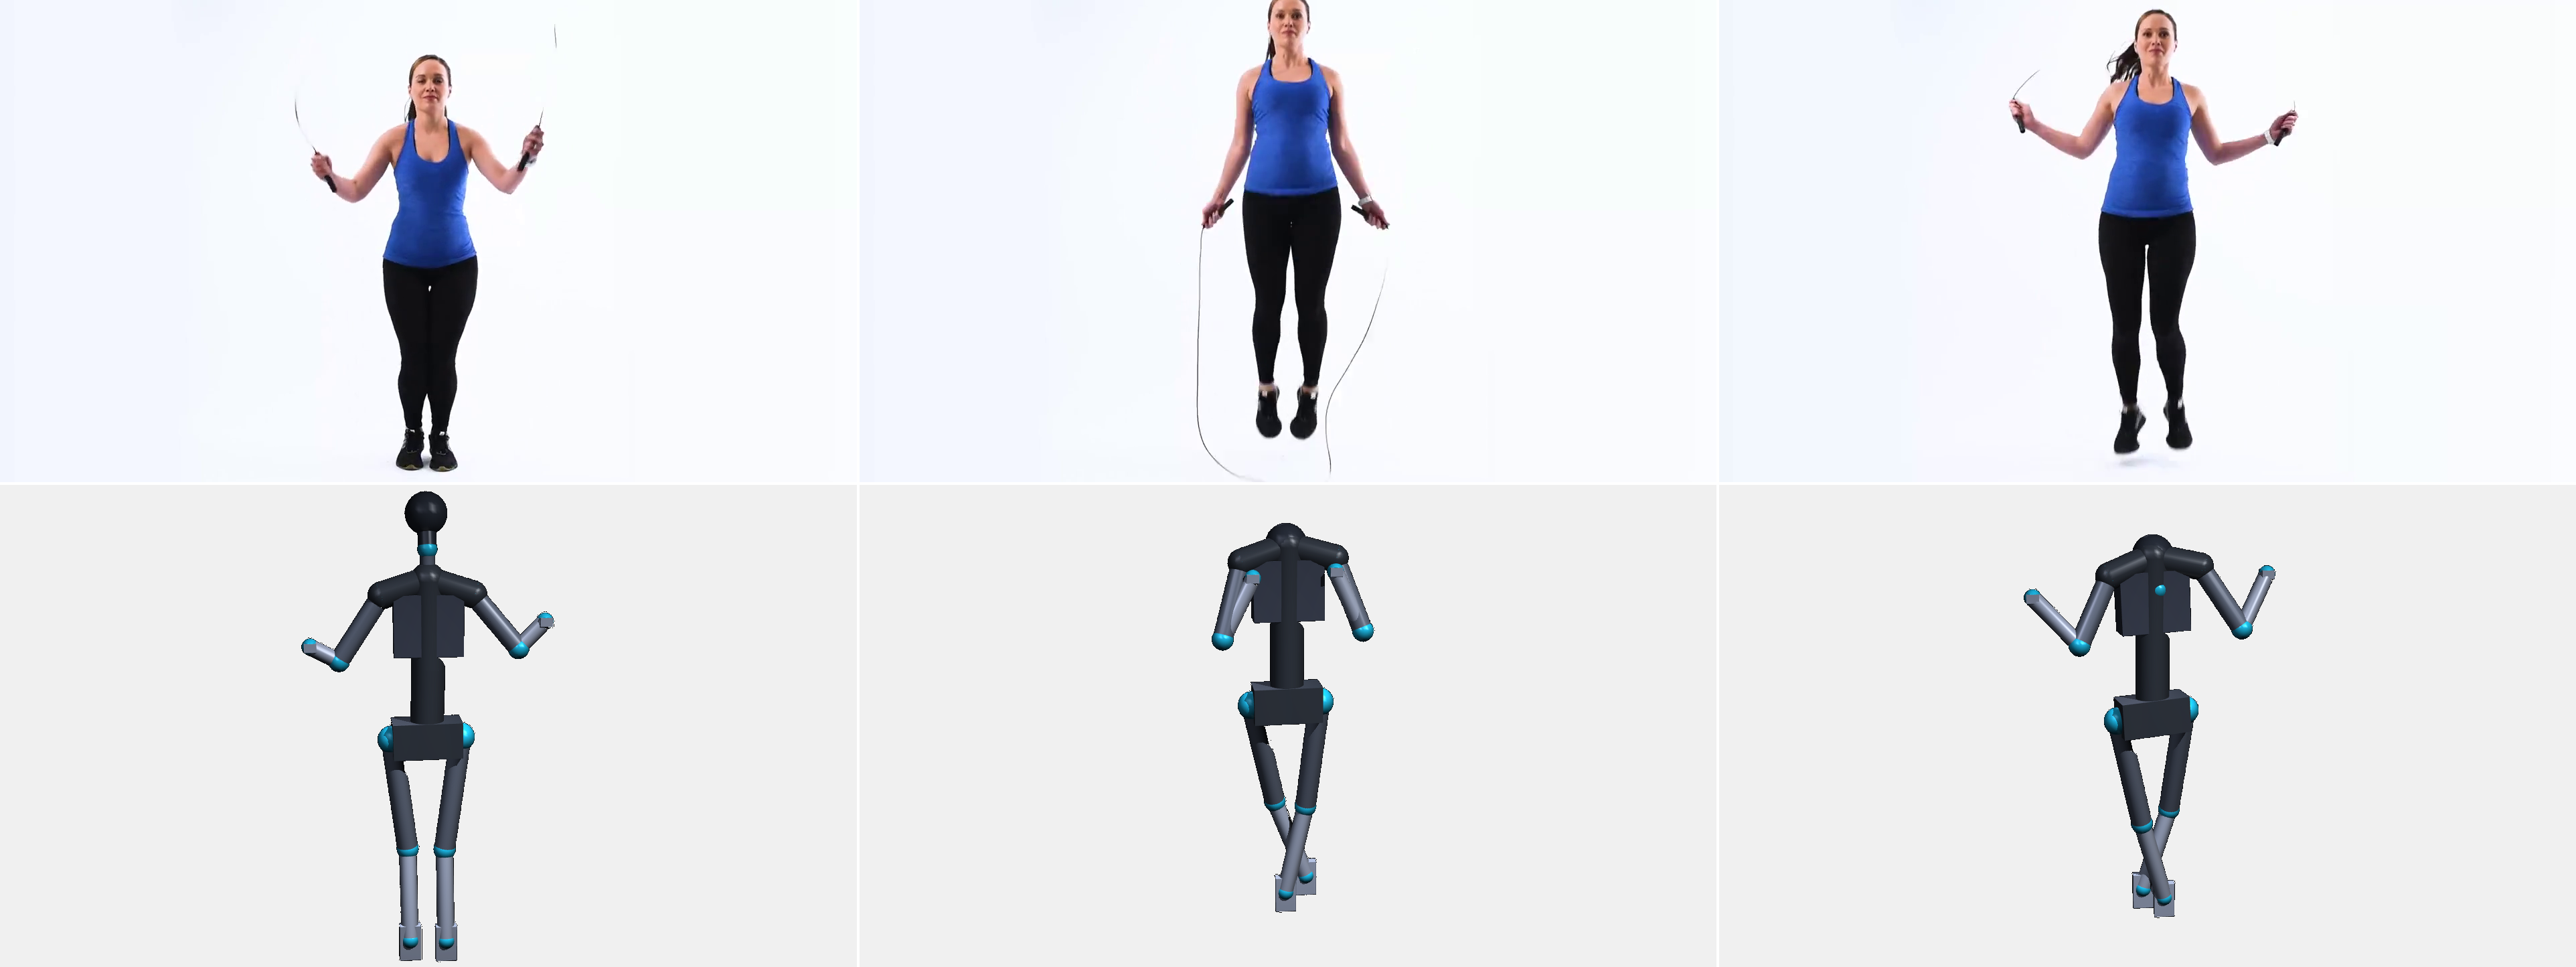
\includegraphics[width=\textwidth]{figures/jump_rope.png}\\[2pt]
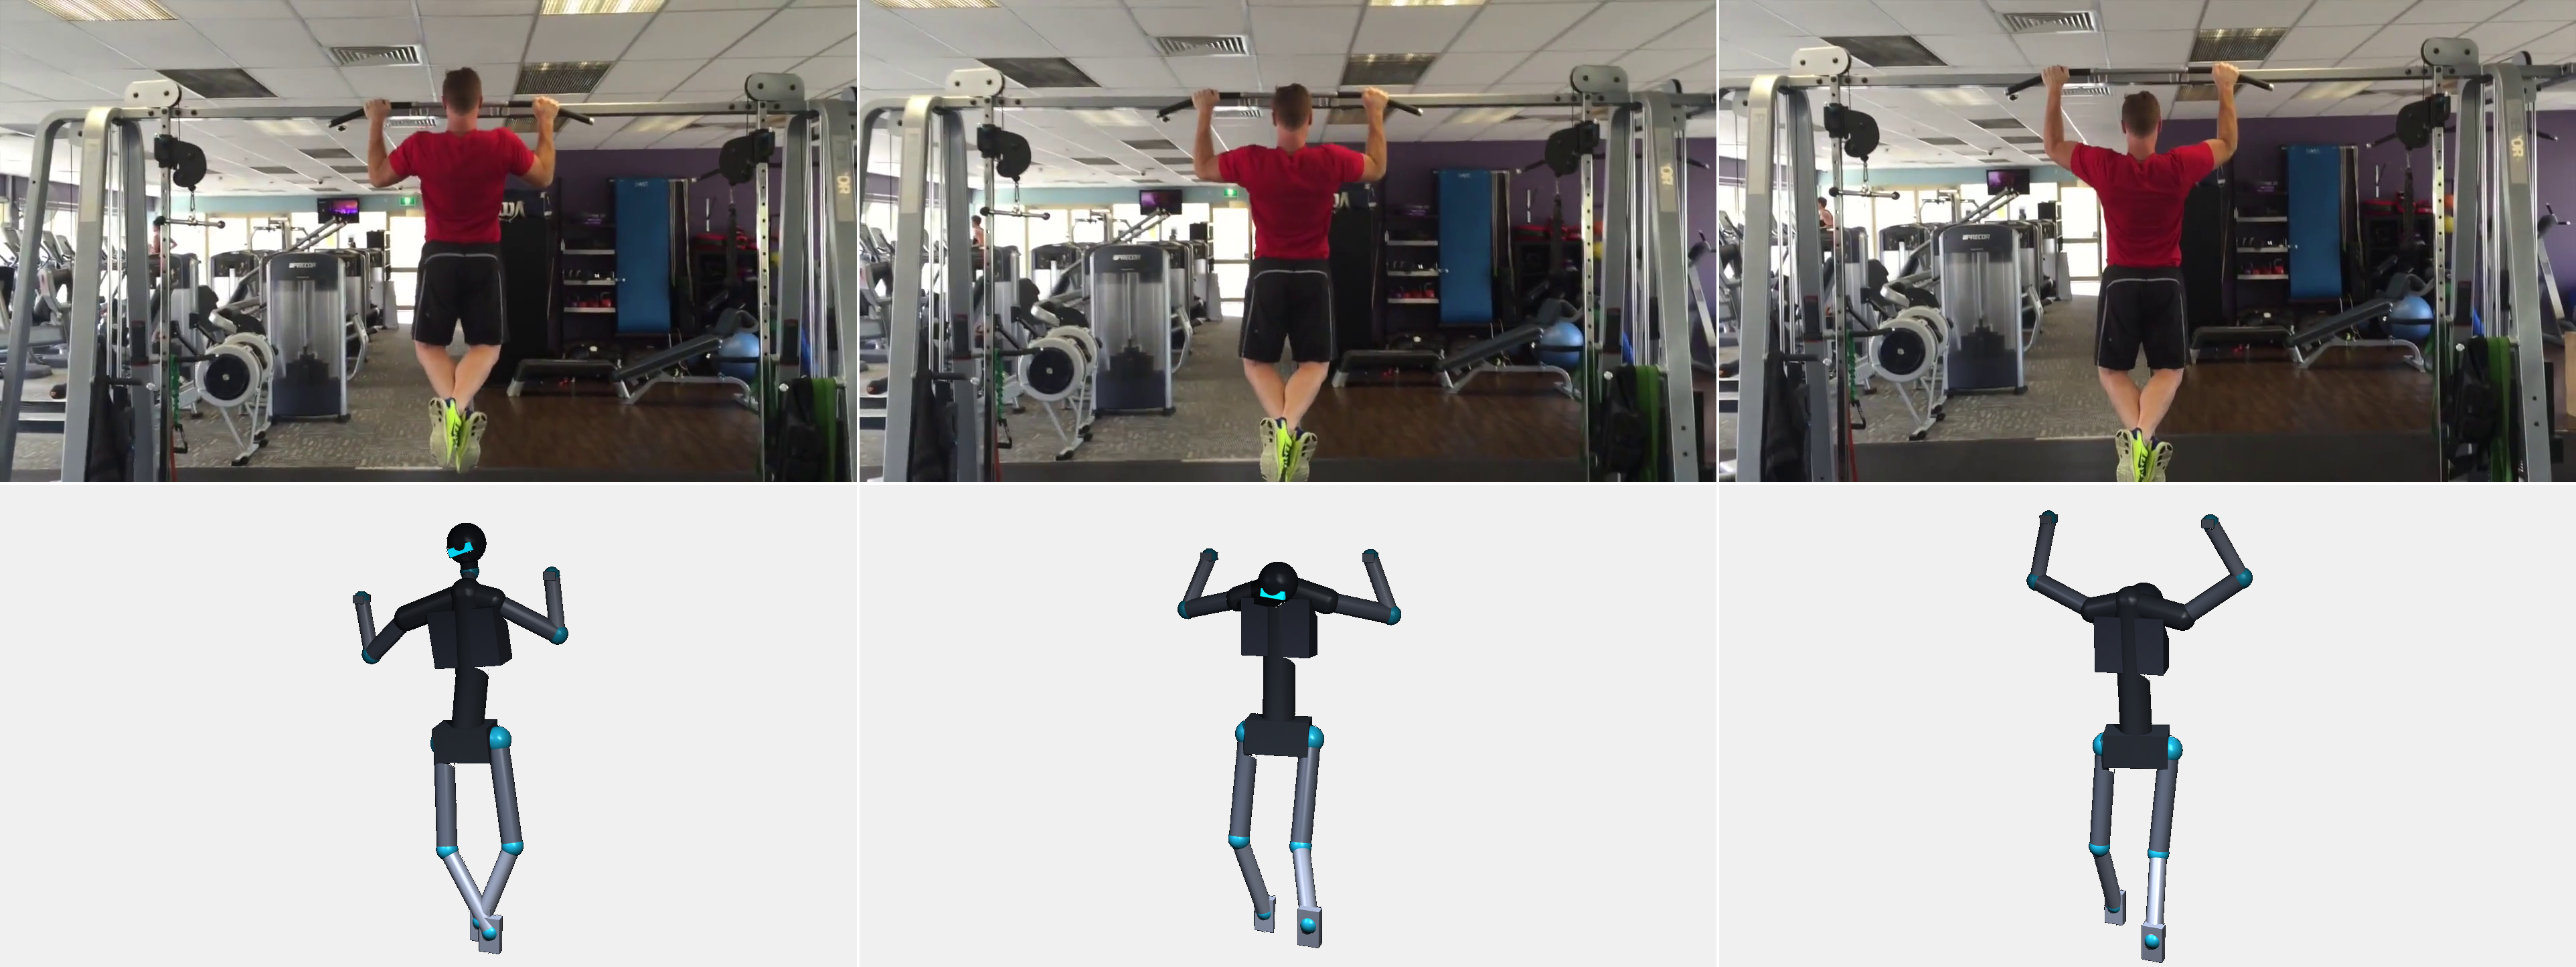
\includegraphics[width=\textwidth]{figures/pull_ups.png}
\caption{Qualitative results on held-out validation clips. Each row shows video frames (top) and the corresponding MuJoCo humanoid rendered from the model's predicted joint angles (bottom) at $t{=}0$, $t{=}7$, and $t{=}15$ of a 16-step (1.6s) trajectory. The robot at $t{=}0$ is initialized from the ground-truth 3D pose; subsequent poses ($t{=}7$, $t{=}15$) are generated via 3-step rolling inference, where the model is re-queried every 3 timesteps with updated visual context. Camera viewpoint is determined by projection-matching the 3D skeleton to the video's 2D keypoints. \textbf{Top:} skipping rope, where the model predicts arm elevation and body compression through the jump cycle (RMSE\,=\,25.1\textdegree). \textbf{Bottom:} pull-ups, where the model tracks the arm extension and hip drop during descent (RMSE\,=\,17.7\textdegree).}
\label{fig:qualitative}
\end{figure*}

Figure~\ref{fig:qualitative} shows two representative examples from the held-out validation set rendered as MuJoCo humanoids. Both clips are cyclical activities (rope-skipping and pull-ups), which is the regime where the model is most accurate. Starting from the ground-truth pose at $t{=}0$, the model's 3-step rolling predictions produce plausible trajectories that track the gross body dynamics: arm elevation and vertical compression in the rope-skipping jump cycle, and arm extension with hip drop during pull-up descent. The largest errors appear in extremities (hands, feet) where kinematic chain errors accumulate.

\textbf{Failure modes.} The model struggles with: (1) fast, discontinuous motions where the 1.6\,s horizon spans qualitatively different poses; (2) compositional multi-step sequences (cooking, sports plays with discrete phases, dance routines) where the next phase is not predictable from current pose alone; (3) fine-grained hand and finger interactions not captured by our 22-DoF representation; (4) activities with significant object interaction where the trajectory depends on object physics. The gap between cyclical and multi-step performance is quantified below in Section~\ref{sec:quantitative} and motivates scaling the pipeline to additional video sources with denser coverage of long compositional actions.

\subsection{Quantitative Evaluation}
\label{sec:quantitative}

We evaluate three trained models under identical protocol: a 325K-clip ablation model trained on the stage-1 intermediate corpus (before re-tracking and VLM judging), MIMIC itself (trained on movement-strict-164), and the 287 model (trained on movement-287). Each model is evaluated on 500 randomly sampled validation clips from the matching split. Given the ground-truth pose at $t{=}0$, each method predicts joint angles for the full 16-step (1.6\,s) action horizon. We report joint-angle RMSE (degrees) on future frames ($t{=}1..15$). We compare against two baselines: \emph{static} (repeat the $t{=}0$ pose for all future frames) and \emph{linear extrapolation} (constant angular velocity from the previous frame). The high-motion subset is the top quartile by total ground-truth angular displacement ($n{=}125$).

\begin{table}[h]
\centering
\caption{Baseline comparison on 500 held-out validation clips per model. Joint-angle RMSE (degrees) on future frames ($t{=}1..15$, 1.5\,s of prediction). The 325K ablation model is trained on the unfiltered intermediate corpus and is reported for comparison; the two released models are trained on the filtered subsets and evaluated on each subset's own held-out validation split.}
\label{tab:baselines}
\begin{tabular}{lcc}
\toprule
\textbf{Method} & \textbf{All} & \textbf{High Motion} \\
\midrule
\multicolumn{3}{l}{\emph{325K stage-1 ablation (unfiltered intermediate corpus):}} \\
Linear baseline & 246.1\textdegree & 366.2\textdegree \\
Static baseline & 43.8\textdegree & 65.6\textdegree \\
325K ablation model & 43.7\textdegree & 63.9\textdegree \\
\midrule
\multicolumn{3}{l}{\emph{movement-strict-164 (released):}} \\
Linear baseline & 188.4\textdegree & 279.1\textdegree \\
Static baseline & 41.0\textdegree & 60.7\textdegree \\
\textbf{MIMIC (strict-164)} & \textbf{39.8\textdegree} & \textbf{57.5\textdegree} \\
\midrule
\multicolumn{3}{l}{\emph{movement-287 (released):}} \\
Linear baseline & 188.8\textdegree & 288.7\textdegree \\
Static baseline & 42.6\textdegree & 65.3\textdegree \\
\textbf{287 model} & \textbf{40.9\textdegree} & \textbf{61.7\textdegree} \\
\bottomrule
\end{tabular}
\end{table}

MIMIC lowers all-clip RMSE by 9\% (43.7\textdegree{} to 39.8\textdegree{}) and high-motion RMSE by 10\% (63.9\textdegree{} to 57.5\textdegree{}) compared to the 325K ablation model. The gap between model and static baseline widens substantially: from 0.1\textdegree{} to 1.2\textdegree{} on all clips (a 12$\times$ larger margin) and from 1.7\textdegree{} to 3.2\textdegree{} on the high-motion subset (5.3\% reduction in error versus 2.6\% in the ablation). This is the strongest signal that the re-tracking and VLM filtering meaningfully improved the training distribution: the model is not just hitting a slightly easier validation set, it is also pulling further ahead of the static reference computed on the same clips.

The 287 model, trained on the broader vlm-good subset that retains lower-motion activities, reaches the same long-horizon RMSE as MIMIC (40.9\textdegree{} vs 39.8\textdegree{} on each model's own val set, near-identical when evaluated on the same val set) but produces sharper short-horizon predictions: step-1 RMSE of 9.6\textdegree{} vs 11.8\textdegree{} for MIMIC, and step-1 median of 2.5\textdegree{} vs 2.9\textdegree{}. We attribute this to broader coverage of low-amplitude motion in the 287 set, which sharpens local pose dynamics without changing the long-horizon ceiling.

\textbf{Per-sample distribution.} For MIMIC at step $S{=}16$, the model achieves median 28.1\textdegree{} (p25\,=\,12.4\textdegree{}, p75\,=\,45.8\textdegree{}), an improvement over the 325K ablation's median of 30.4\textdegree{}. The wide p25 to p75 spread is the most informative number in this section: it reflects a roughly bimodal performance pattern that we discuss in the next paragraph.

\textbf{Cyclical versus multi-step activities.} The model performs substantially better on cyclical or repeated motions than on long compositional sequences. Pull-ups, squats, jumping jacks, jumping rope, and similar repeating motions cluster in the p25 tail (well below 12\textdegree{}), where the relationship between the visible posture phase and the next 1.6\,s is largely periodic and recoverable from a short observation window. Multi-step activities, in contrast, cluster in the p75 tail. Cooking sequences, assembly tasks, sports plays with discrete phases (the windup, throw, and follow-through of a baseball pitch), and dance routines all involve choices that are not predictable from current pose alone over a 1.5\,s window, and the model has limited training signal for the long-horizon transitions that distinguish them. We read this as a data-coverage limitation rather than a model-capacity ceiling: the DiT scaling table (Section~\ref{sec:scaling}) showed plateauing returns to parameters at the current data scale, and the gap between cyclical and multi-step performance is exactly the gap that more (and longer-horizon) coverage of compositional human activity would address. Datasets such as Ego4D, HowTo100M, and InternVid contain orders of magnitude more such material and our pipeline can ingest them without modification.

\textbf{Linear extrapolation} continues to degrade catastrophically over the 1.5\,s horizon: while its short-horizon error is small, the constant-velocity assumption drives predictions far outside the valid joint-angle range as the horizon grows. Because our evaluation setting (22-DoF joint angle prediction from monocular video with language conditioning) is novel, there are no directly comparable published baselines; the closest systems (GR00T N1--N1.6, Helix) evaluate on physical robots with different action spaces.

%==============================================================================
\section{Limitations and Future Work}
\label{sec:limitations}
%==============================================================================

\textbf{Scaling Data and Training.} Kinetics-700 represents a fraction of available internet video. Datasets like Ego4D, HowTo100M, and InternVid offer orders-of-magnitude more coverage, including the long compositional activities where our model is weakest. The bimodal performance split between cyclical and multi-step motion (Section~\ref{sec:quantitative}) is consistent with a data-coverage limitation rather than a model-capacity ceiling: DiT scaling already showed diminishing returns at the current data scale (Table~\ref{tab:scaling}), and the p75 of our error distribution corresponds almost entirely to compositional sequences that have only sparse representation in Kinetics-700. Our pipeline is fully automated and can ingest these additional sources without modification, including the second-stage re-tracking and VLM judging.

\textbf{Simulation Deployment.} We lack physical humanoid hardware. Emerging simulation environments (MuJoCo Playground, Isaac Lab, Genesis) would enable closed-loop evaluation, testing whether the model can correct for drift, respond to perturbations, and produce physically stable gaits.

\textbf{Hand Articulation.} Our 22-DoF representation excludes hand and finger articulation. Integrating egocentric hand-tracking datasets could extend coverage to dexterous manipulation.

\textbf{Action Frequency.} At 10Hz, our model is slower than Helix (200Hz) or $\pi_0$ (50Hz). Temporal upsampling or hierarchical prediction could increase frequency for dynamic tasks.

\textbf{Angle Representation.} Sin/cos pairs avoid discontinuities at $\pm\pi$ but double dimensionality (22 to 44). More compact representations like 6D rotation~\cite{zhou2019continuity} could reduce this for 3-DoF ball joints.

%==============================================================================
\section{Conclusion}
%==============================================================================

We have presented MIMIC, an open-source vision-language-action model for full-body humanoid control, trained on movement-strict-164 entirely from internet human video. Our two-stage data pipeline combines deterministic pose extraction and quality filters with a re-tracking pass and a 235B VLM judge, producing two distributable training sets: movement-strict-164 (164K clips, our highest-quality release used for MIMIC) and movement-287 (287K clips, broader motion coverage, used to train a sibling model). Our key findings are: (1) the GR00T N1-style dual-system architecture transfers effectively to human video data, requiring no robotic teleoperation; (2) DiT scaling yields consistent improvements up to $\sim$1.3B parameters, with diminishing returns beyond; (3) continuous angle representations (sin/cos pairs) are essential for stable training; (4) the second-stage re-tracking and VLM-judged filtering reduces validation RMSE by roughly 10\% and widens the model-versus-static gap by an order of magnitude on the same architecture; (5) the model is substantially more accurate on cyclical or repeating activities than on long multi-step compositional sequences, a gap we attribute to dataset coverage rather than model capacity and which motivates ingesting additional video sources; and (6) the entire system (data processing, re-tracking, VLM judging, training, and inference) runs on consumer GPUs. By releasing both filtered datasets, model weights, and all training, re-tracking, and judging code, we lower the barrier to entry for humanoid VLAM research from expensive robotic infrastructure to internet-scale video processing on a single workstation. The most important next step is deployment in simulation and on physical hardware to evaluate the model in true closed-loop settings with environmental feedback.

%==============================================================================
\section*{Data and Code Availability}
%==============================================================================

All resources are publicly available:
\begin{itemize}
    \item \textbf{Code:} \url{https://anonymous.4open.science/r/movement-D88C}
    \item \textbf{Dataset (movement-strict-164):} anonymized for review
    \item \textbf{Dataset (movement-287):} anonymized for review
    \item \textbf{Model weights (MIMIC):} anonymized for review
\end{itemize}

% De-anonymized URLs (for camera-ready version):
% Code:                 https://github.com/maxsegan/movement
% Dataset (strict-164): https://huggingface.co/datasets/maxsegan/movement-strict-164
% Dataset (287):        https://huggingface.co/datasets/maxsegan/movement-287
% Model:                https://huggingface.co/maxsegan/mimic-vlam

%==============================================================================
\section*{Acknowledgments}
%==============================================================================

This work was supported in part by the U.S. National Science Foundation AI Institute for Dynamical Systems, grant \#2112085 to [redacted for review]. We acknowledge the Kinetics-700 dataset, and the authors of ViTPose, MotionAGFormer, and Qwen3-VL for releasing pretrained models and code, and Anthropic for Claude Code, which was used in this work.

%==============================================================================
\bibliographystyle{plain}
\begin{thebibliography}{99}

\bibitem{rt2}
Brohan et al. RT-2: Vision-Language-Action Models Transfer Web Knowledge to Robotic Control. CoRL 2023.

\bibitem{openvla}
Kim et al. OpenVLA: An Open-Source Vision-Language-Action Model. CoRL 2024.

\bibitem{pi0}
Physical Intelligence. $\pi_0$: A Vision-Language-Action Flow Model for General Robot Control. 2024.

\bibitem{groot}
NVIDIA. GR00T N1: An Open Foundation Model for Generalist Humanoid Robots. 2025.

\bibitem{groot_n15}
NVIDIA. GR00T N1.5: Advancing Generalist Humanoid Robot Capabilities. 2025.

\bibitem{groot_n16}
NVIDIA. GR00T N1.6: Building Generalist Humanoid Capabilities with Sim-to-Real Workflows. 2025.

\bibitem{helix}
Figure AI. Helix: A Vision-Language-Action Model for Generalist Humanoid Control. 2025.

\bibitem{octo}
Team et al. Octo: An Open-Source Generalist Robot Policy. RSS 2024.

\bibitem{tinyvla}
Wu et al. TinyVLA: Efficient Vision-Language-Action Models. 2024.

\bibitem{motiongpt}
Jiang et al. MotionGPT: Human Motion as a Foreign Language. NeurIPS 2023.

\bibitem{motiondiffuse}
Zhang et al. MotionDiffuse: Text-Driven Human Motion Generation with Diffusion Model. 2022.

\bibitem{uh1}
Wang et al. UH-1: A Universal Humanoid Model for Full-Body Control from Text. 2024.

\bibitem{r3m}
Nair et al. R3M: A Universal Visual Representation for Robot Manipulation. CoRL 2022.

\bibitem{egovla}
EgoVLA: Egocentric Video Pretraining for Vision-Language-Action Models. 2025.

\bibitem{mimicvideo}
mimic-video: Scaling Internet Video Pretraining for Robotic Manipulation. 2025.

\bibitem{wholebodyvla}
WholeBodyVLA: Whole-Body Vision-Language-Action Model from Action-Free Egocentric Video. 2025.

\bibitem{sonic}
SONIC: Scaling Motion Tracking for Natural Humanoid Control. 2025.

\bibitem{ntu120}
Liu et al. NTU RGB+D 120: A Large-Scale Benchmark for 3D Human Activity Understanding. TPAMI 2020.

\bibitem{bytetrack}
Zhang et al. ByteTrack: Multi-Object Tracking by Associating Every Detection Box. ECCV 2022.

\bibitem{vitpose}
Xu et al. ViTPose: Simple Vision Transformer Baselines for Human Pose Estimation. NeurIPS 2022.

\bibitem{motionagformer}
MotionAGFormer: Attention-based Graph Transformer for Human Motion Prediction. 2023.

\bibitem{qwen3vl}
Bai et al. Qwen3-VL Technical Report. 2025.

\bibitem{flowmatching}
Lipman et al. Flow Matching for Generative Modeling. ICLR 2023.

\bibitem{pi05}
Physical Intelligence. $\pi_{0.5}$: A Vision-Language-Action Model with Open-World Generalization. arXiv 2504.16054, 2025.

\bibitem{pi0fast}
Physical Intelligence. FAST: Efficient Action Tokenization for Vision-Language-Action Models. 2025.

\bibitem{gemini15}
Google DeepMind. Gemini Robotics 1.5: Motion Transfer and Multi-Embodiment Learning. 2025.

\bibitem{smolvla}
Hugging Face. SmolVLA: A Small Vision-Language-Action Model for Efficient Robot Control. 2025.

\bibitem{openvla_oft}
Kim et al. OpenVLA-OFT: Open Vision-Language-Action Models with Optimal Fine-Tuning. 2025.

\bibitem{a2a}
Luo et al. Action-to-Action: Single-Step Flow Matching for Robot Control. 2025.


\bibitem{zhou2019continuity}
Zhou et al. On the Continuity of Rotation Representations in Neural Networks. CVPR 2019.

\end{thebibliography}

\end{document}
